% Encoding: UTF-8
\documentclass[final,bibliography=totocnumbered]{include/sikseminar}
\usepackage[utf8]{inputenc}
\usepackage[textsize=tiny]{todonotes}
\usepackage{hyperref}
\usepackage[T1]{fontenc}
\usepackage[inline]{enumitem}
\usepackage[autostyle=true,german=quotes]{csquotes}
\usepackage{subcaption}
\usepackage{xspace}

\usepackage{tabu}
\tabulinesep=1.2mm

\usepackage[acronym,toc,section=section,numberedsection,nomain]{glossaries}
\newacronym[shortplural={CPS},longplural={Cyber-physical Systems}]{cps}{CPS}{Cyber-physical System}


\hypersetup{colorlinks = true,linkcolor = black,citecolor = black,urlcolor = black,filecolor = black}

\usetikzlibrary{shapes.geometric}
\graphicspath{{./figure/}}
\bibliography{bib/cps}

\clubpenalty=10000
\widowpenalty=10000
\overfullrule=1mm

\newcommand{\fb}[1]{\dofb#1}
\newcommand{\cps}{\glspl{cps}\xspace}
\newcommand{\dofb}[1]{\textbf{#1}\nobreak\hspace{0pt}}

\begin{document}


    \Title[Security Considerations for \glsentrytext{cps}]{Security Considerations for Cyber-Physical Systems}
    \makeTitle

    \Author{Maximilian Ammann}
    \Studiengang{Bachelor Informatik}
    \makeAuthor
    \date{Datum des Vortrags \todo}
    \subject{Seminar Cyber-Physical Systems}

    \maketitle

    \begin{abstract}
        \section*{Kurzfassung}
        Durch die enge Koppelung von physischen und Cyber-System bei \cps ergeben sich neue relevante Eigenschaften, welche eine Erweiterung der Eigenschaften von klassischen Systemen darstellen.

        Zahlreiche Angriffe belegen die mangelhafte Sicherheit von derzeitig eingesetzten \cps.
        Deshalb soll in dieser Arbeit ein Überblick über potentielle Angreifergruppen und Angriffsszenarien gegeben werden, um adäquate Gegenmaßnahmen vorzustellen.
        Gegenmaßnahmen können dabei sowohl proaktiv als auch reaktiven eingesetzt werden, um \cps zu schützen.

        Zuletzt soll diskutiert werden in wie fern momentan eingesetzte Systeme, in Bezug auf Sicherheit, verbessert werden können.

    \end{abstract}
    \todo{
    Sind alle Begriffe definiert und klar?
    }
    \thispagestyle{empty}
    \newpage
    \tableofcontents
    \newpage

    \section{Einführung}
    \label{sec:intro}
    \cps sind meist eingebettete Echtzeitsysteme, welche eine hohe Verfügbarkeit, Robustheit, Widerstandsfähigkeit und Berechenbarkeit aufweisen müssen.
    Die physische Welt macht hohe Verfügbarkeit allerdings oft schwierig, da sie alles andere als berechenbar ist~\cite{Lee08,SGL+08}.
    Einsatzorte für diese Systeme sind beispielsweise intelligente Stromnetze, symbiotische Sensornetzwerke für die Agrarwirtschaft und Katastrophenabwehr, medizinische oder assistierende Geräte, intelligente Verkehrssteuerung, intelligente Gebäude~\cite{RLS+10}, Autos und \glspl{ics} sein~\cite{HLL+17}.

    In diesen Beispielen spielt ein außerordentliches Maß an Vertrauen eine Rolle~\cite{SGL+08}.
    Dieses ist zwar auch bei Cyber-Systemen gefordert, allerdings ohne die Koppelung an physische Prozesse~\cite{BG11}.
    Zudem unterliegt man konzeptionell bedingt auch einigen Restriktionen wie beispielsweise die Bindung an eine Batterie oder eine leichte Bauweise~\cite{YWY+17}.
    Es existiert also ein Unterschied zwischen den Anforderungen an \cps und Cyber-Systemen, wie Anwendungsservern oder Heimcomputern, sodass man diese in Bezug auf Sicherheit auf einem anderen Blickwinkel betrachten muss.

    In dem Kapitel~\ref{sec:bedeutung-sicherheit} wird zunächst das Zusammenspiel von physischen und Cyber-Systemen im Bezug auch Sicherheit geklärt.
    Zudem werden mögliche Angreifer in Kapitel~\ref{subsec:angreifergruppen} beleuchtet.
    In Kapitel~\ref{sec:angriffszenarien} werden mögliche Szenarien für Angriffe und in Kapitel~\ref{sec:gegenmassnahmen} dazu Gegenmaßnahmen dargestellt.
    Zuletzt soll in Kapitel~\ref{sec:improve-security-situation} diskutiert werden, wie die aktuelle Sicherheitssituation verbessert werden kann.
    % Beispiele:
    %   Stuxnet (Langer)
    %   Spectre: https://arxiv.org/pdf/1811.05441.pdf
    %   EU: https://eur-lex.europa.eu/legal-content/EN/TXT/?uri=JOIN:2017:0450:FIN https://ec.europa.eu/transport/sites/transport/files/3rd-mobility-pack/com20180283_en.pdf
    %   https://nakedsecurity.sophos.com/2018/11/15/darpa-uses-a-remote-island-to-stage-a-cyberattack-on-the-us-power-grid/?utm_campaign=Security%2BNewsletter&utm_medium=email&utm_source=Security_Newsletter_co_103

    \section{Bedeutung von Sicherheit in \glsentrytext{cps}}
    \label{sec:bedeutung-sicherheit}

    Die Eigenschaften von Cyber-Systemen und physischen Systemen in Bezug auf Sicherheit unterscheiden sich.
    Deshalb soll im Folgenden Sicherheit speziell für \cps definiert werden.

    \subsection{Sicherheitsrelevante Eigenschaften von \glsentrytext{cps}}
    \label{subsec:definition}
    Unter Sicherheit bei Cyber-Systemen versteht man im Allgemeinen Informationssicherheit.
    Informationssicherheit kann man durch drei Eigenschaften von Systemen charakterisieren~\cite{CH13}:
    \begin{itemize}[noitemsep,wide=0pt]
        \item \fb{Confidentiality} - Nur autorisierte Teilnehmer können auf Ressourcen zugreifen.
        \item \fb{Integrity} - Ressourcen können nur von autorisierten Teilnehmern verändert werden.
        \item \fb{Availability} - Ressourcen ist für autorisierte Teilnehmer angemessen verfügbar.
    \end{itemize}

    Zwischen diesen drei Eigenschaften muss bei der Entwicklung ein sinnvolles Gleichgewicht gefunden werden.
    \citeauthor{GK16}~\cite{GK16} beschreiben, dass bei Cyber-Systemen der Fokus auf \textit{Confidentiality} (dt.\ Vertraulichkeit) und bei \cps eher auf \textit{Availability} (dt.\ Verfügbarkeit) liegt.
    Dieser Fokus ist kritisch zu betrachten, wenn man die diversen Einsatzorte und sicherheitskritischen Anforderungen von \cps betrachtet.

    Sie schlagen außerdem vor das CIA-Dreieck\todo{Erklären} im Hinblick auf \cps durch die Eigenschaft \textit{Veracity} (dt.~Richtigkeit) zu erweitern.
    Ein System hat diese Eigenschaft genau dann, wenn Aussagen des Systems die Wahrhaftigkeit der Wirklichkeit reflektieren.
    Es muss also sichergestellt werden, dass Sensoren, durch beispielsweise physische Maßnahmen (siehe Kapitel~\ref{physisch-orga}) fälschungssicher sind.
    Confidentiality und Integrity (dt.\ Integrität) sind nicht ausreichend um die Richtigkeit von Informationen zu garantieren.
    Veracity ist eine relativ starke Eigenschaft.
    Deshalb kann man in Fällen, in denen diese nur schwer zu erreichen ist, zunächst auf Plausibility setzen.
    Herbei hat ein System genau dann diese Eigenschaft, wenn Aussagen des Systems nicht zu weit von erwartbaren Werten abweichen.
    Liefert ein Sensor beispielsweise einen für physikalische Modelle unmögliche Wert, so ist dieser nicht plausibel und das System kann dies als möglichen Angriff erkennen.~\cite{GK16}

    Diese Eigenschaft kann nicht durch Integrity gewährleistet werden, da die Werte eines Sensors von außerhalb des \cps beeinflusst werden können.
    Veracity stellt also eine grundsätzlich andere Eigenschaft bereit.

    \citeauthor{WYX+10}~\cite{WYX+10} und \citeauthor{SFJ17}~\cite{SFJ17} stimmen zu, dass eine Überprüfung auf die Richtigkeit von Informationen wichtig sind.
    Sie erweitern das CIA-Dreieck zudem um die Eigenschaft der \textit{Authenticity} (dt.\ Authentizität) zwischen Kommunikationspartnern.
    Authenticity kann genau dann hergestellt werden, wenn sich beide Kommunikationspartner einig über die Identität des Gegenübers sind~\cite{CH13}.
    %Obwohl bei der Definition von \citeauthor{CH13} die Authenticity bereits in der Definition beinhaltet ist, soll diese hier dennoch zusätzlich aufgeführt werden.
    Es könnte behauptet werden, dass sich Integrity und Authenticity decken.
    Daten können allerdings Integrity durch z.B.\ Prüfsummen und gleichzeitig keine Authenticity besitzen.
    In der Realität bringt Authenticity aber oftmals Integrity mit sich.

    Ein weiteres wichtiges Konzept ist die \textit{Non-repudiation} (dt.\ Revisionssicherheit).
    Hierbei muss das System das Eintreten jeglicher Ereignisse und dessen Auslöser oder Teilnehmer nachvollziehbar machen \cite{CH13}.
    %Hierbei darf es nicht möglich sein aufgezeichnete Aktionen zu leugnen \cite{NIST2013}.
    Ein System hat diese Eigenschaft also genau dann, wenn jedes Ereignis, welches das System beeinflusst, nachvollzogen werden kann.

    \begin{figure}[h]
        \centering
        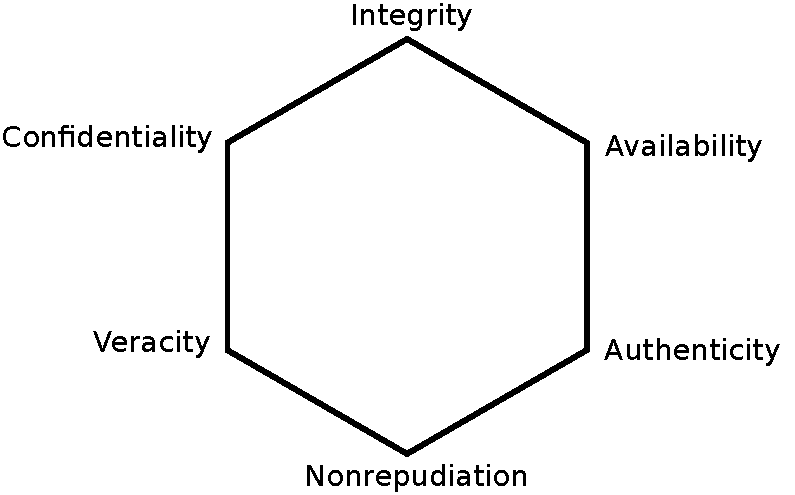
\includegraphics[height=4cm]{triad}
        \caption{Erweitertes CIA-Dreieck}
        \label{fig:triad}
    \end{figure}

    Die Eigenschaften von Systemen aus der klassischen Informationssicherheit sind also nicht ausreichend um das oft komplexe Zusammenspiel von physischen- und Cyber-Systemen\todo{physischen- richtig?} abzusichern.
    Bei \cps ist also sowohl die Richtigkeit von Informationen als auch die zweifelsfreie Identifikation zweier Parteien wichtig.
    Deshalb sind zusätzliche Eigenschaften wie Veracity und Authenticity, wie in Abbildung~\ref{fig:triad} zu sehen ist, nötig um die Sicherheitsbedürfnisse von \cps abzudecken.
    \citeauthor{CH13}~\cite{CH13} führt noch weitere Eigenschaften wie Accountability, Auditability und Privacy auf, welche allerdings in dieser Arbeit nicht weiter untersucht werden sollen.\todo{Erklären warum nicht (Platzgründe genügt.)}

    \todo{Tabelle mit Eigenschaften}


    \begin{figure}[h]
        \centering
        \begin{longtabu}
            to \linewidth { | l | X[6,l] | X[1.2,l] | }
            \hline
            Eigenschaft&Ein System hat diese Eigenschaft genau dann, wenn~\ldots&Relevante Literatur \\
            \hline
            Confidentiality&
            \ldots nur autorisierte Teilnehmer auf Ressourcen zugreifen können.&
            \cite{CH13} \\
            \hline
            Integrity&
            \ldots Ressourcen nur von autorisierten Teilnehmern verändert werden können.&
            \cite{CH13} \\
            \hline
            Availability&
            \ldots Ressourcen für autorisierte Teilnehmer angemessen verfügbar ist.&
            \cite{CH13} \\
            \hline
            Veracity &
            \ldots Aussagen des Systems die Wahrhaftigkeit der Wirklichkeit reflektieren.&
            \cite{KLG15} \cite{GK16}\\
            \hline
            Authenticity&
            \ldots sich beide Kommunikationspartner einig über die Identität des Gegenübers sind.&
            \cite{SFJ17} \cite{CH13}\\
            \hline
            Non-repudiation &
            \ldots jedes Ereignis, welches das System beeinflusst, nachvollzogen werden kann.&
            \cite{CH13} \cite{SFJ17} \cite{Ross15} \\
            \hline
        \end{longtabu}
        \caption{Übersicht der \cps Eigenschaften}
        \label{fig:table}
    \end{figure}

    % Begriffe: computer, information, network, communication, physical security


    \subsection{Angreifergruppen}
    \label{subsec:angreifergruppen}

    Angriffe können von unterschiedlichen Gruppen aus unterschiedlichen Gründen ausgehen.
    Im Folgenden sollen verschiedene Gruppen nach den Faktoren
    \begin{enumerate*}[label=(\alph*),before=\unskip{: }, itemjoin={{; }}, itemjoin*={{, und }}]
        \item Angreifergruppe\label{factor:angreifergruppe}
        \item Angriffsziel\label{factor:target}
        \item Motiv\label{factor:motiv}
        \item Angriffsvektoren\label{factor:methode}
        \item Konsequenzen\label{factor:konsequenz}
    \end{enumerate*} aufgezählt werden~\cite{HLL+17}.\todo{Aufzählung entfernen?}

    Kriminelle Gruppen \ref{factor:angreifergruppe} versuchen oft mit Hilfe von Erpressung \ref{factor:methode} ein Ziel anzugreifen \cite{WYX+10}.
    Dabei sind Cyberangriffe nur ein logischer nächster Schritt der Kriminellen, da diese weitaus günstiger, weniger riskant, nicht durch Entfernungen eingeschränkt und einfacher zu koordinieren und wiederholen sind. \cite{CAS+09}

    Computerforensiker~\ref{factor:angreifergruppe} haben nicht unbedingt als Ziel selbst ein System zu beschädigen.
    Zum einen kann das Finden von Lücken als Ziel haben, diese unter bestimmten Auflagen offen zulegen oder schließen zu können~\ref{factor:motiv}. \todo{Zitat fehlt}
    Zum anderen können diese aber auch als Schadsoftware verkaufen werden~\ref{factor:motiv}. \todo{Zitat fehlt}

    Unzufriedene Mitarbeiter~\ref{factor:angreifergruppe} eines Unternehmens haben viel Wissen über dessen Infrastruktur.
    Das Ziel ist hierbei die Schädigung des Unternehmens~\ref{factor:konsequenz}.
    Zudem existiert eventuell Zugriff auf das System, sodass überhaupt kein Umgehen von Sicherheitsmechanismen notwendig ist~\ref{factor:methode}.~\cite{CAS+09,WYX+10}

    Aktivistische Gruppierungen~\ref{factor:angreifergruppe} zielen oft auf kritische \cps~\ref{factor:target}, wie beispielsweise Kernkraftwerke oder \gls{scada} Systemen in Fabriken, ab, um diese zu manipulieren~\cite{CAS+09,HLL+17}. \todo{Spionage?}
    Damit dies erreicht werden kann, existiert die Möglichkeit Forensiker oder Insider zu engagieren~\ref{factor:methode}.~\cite{WYX+10}

    Staaten~\ref{factor:angreifergruppe} können politisches und militärisches Interesse~\ref{factor:motiv} daran haben Infrastruktur innerhalb oder außerhalb des Staatsgebiets~\ref{factor:target} anzugreifen \cite{CAS+09}, um diese zu sabotieren oder auszuspionieren.
    Auch hier können Forensiker oder Insider engagiert werden~\ref{factor:methode}.

    Das Wissen über den Angreifer und dessen Motivation kann maßgeblich bei der Wahl und der Strategie der Gegenmaßnahmen helfen.
    Zudem können, wie im nächsten Kapitel beschrieben, dadurch Gefahrenmodelle\todo{Noch relevant?} und detailliertere Angriffsszenarien entworfen werden.

    \section{Angriffsszenarien}
    \label{sec:angriffszenarien}
    % Confidentiality, Integrity, Availability, Veracity
    \begin{figure}
        \centering
        \begin{subfigure}[b]{0.3\textwidth}
            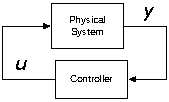
\includegraphics[width=\textwidth]{abstrakt}
            \caption{Ohne Angriffspunkte}
            \label{fig:abstrakt}
        \end{subfigure}
        \qquad
        \begin{subfigure}[b]{0.4\textwidth}
            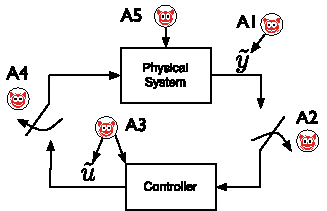
\includegraphics[width=\textwidth]{attack_points}
            \caption{Mit Angriffspunkten}
            \label{fig:attack_points}
        \end{subfigure}
        \caption{Abstraktion eines \cps~\cite{CAS08}}
    \end{figure}

    In Abbildung~\ref{fig:abstrakt} ist eine abstrakte Darstellung eines \cps zu sehen.
    Der \enquote{Controller} sendet Befehle über $u$ an das \enquote{Physical System}.
    Dieses wiederum schickt Resultate oder Sensorwerte über $y$ an den \enquote{Controller}.
    In Abbildung~\ref{fig:attack_points} sind mögliche Angriffspunkte dargestellt.
    Hierbei stellen A1 und A3 \gls{mitm} dar, A4 und A2 \gls{dos} und A5 einen physischen Angriff.
    Im folgenden Kapitel sollen Angriffe an verschiedenen Punkten eines \cps dargestellt werden.

    % Sabotage und Spionage
    % Migration von Legacy Systemen ist kritisch (Gollman, 1.)
    % Unterschied zu Cyber-Systemen (Cardenas 2008, 3.)
    % IoT Unterschiede zu Cyber-Systemen (FPA+18)
    % Workflow von CPS (WYX+10, II.)

    \subsection{\glsentrylong{dos} Angriff}
    \label{subsec:dos}
    \gls{dos} Angriffe zielen darauf ab das Cyber-System mit einer großen Flut an Informationen zu stören.
    Diese können von einem angeschlossenes Netzwerk oder dem physischen System ausgehen.\todo{missing cite}
    Dadurch wird der Informationsfluss von Steuer- und Nutzdaten, wie in Abbildung~\ref{fig:attack_points} an den Punkten A4 und A2 zu sehen ist, unterbrochen und die Availability des \cps eingeschränkt.

    Diese Angriffe sind beispielsweise bei CAN Bussen in Autos realistisch, da Nachrichten mit vielen Empfängern gesendet werden~\cite{KCR+10} und auch die Fehlerbehebung angreifbar ist~\cite{CDV13}.
    % Koscher2010: Konkret wurde der Tacho auf 0 gesetzt
    Folgen können sein, dass sich Fenster nicht mehr schließen lassen und Warnlichter oder die Diebstahlsicherung deaktiviert werden können~\cite{HKD08}.

    Auch in echtzeitkritischen intelligenten Stromnetzen kann ein massives Überfluten dazu führen, dass der Normalbetrieb nicht mehr möglich ist~\cite{LLW+10}.
    Der Einsatz von kabelloser Kommunikation erhöht dabei das Angriffspotential~\cite{LWW11}\todo{check cite}, da diese allgemein eine geringere Bandbreite aufweisen.

    % Distributed DoS

    \subsection{\glsentrylong{mitm} Angriff}
    \label{subsec:mitm}
    % Unterschied Active vs Passive: http://www.security-science.com/pdf/active-man-in-the-middle.pdf
    Bei \gls{mitm} Angriffe kann man zwischen aktiven und passiven Angriffen unterscheiden~\cite{WYX+10}.
    Passive verändern den Netzwerkverkehr nicht, sondern lauschen nur um an Informationen zu gelangen (sog.\ Lauschangriff).
    Hierbei wird die Confidentiality von Daten missachtet.

    Bei aktiven hingegen wird der Verkehr zwischen zwei Kommunikationspartnern zudem noch verändert.
    Beide Arten nutzen allerdings dieselben initialen Angriffsvektoren.
    In der Abbildung~\ref{fig:attack_points} stellt A1 und A3 aktive \gls{mitm} Angriffe dar.
    Ein Controller kommuniziert über ein Netzwerk mit einem physischen System über die Verbindungen $y$ und $u$.
    Ziel eines Angreifers ist es den Netzwerkverkehr zwischen den beiden anderen Hosts über sich zu leiten~\cite{WYX+10,FPA+18} um ihn so beeinflussen zu können.
    In der Abbildung ist dies dadurch dargestellt, dass $y \ne \tilde{y}$ und $u \ne \tilde{u}$.
    Ein passiver Angriff die Kommunikation nicht verändern, dh.\ es gilt $y = \tilde{y}$ und $u = \tilde{u}$.
    Diese Angriffe können also aufgrund von fehlender Authenticity zu einem Verlust von Integrity führen, da nicht sichergestellt ist, dass die Daten nicht manipuliert wurden.\todo{Mehr erklären?}

    Dies ist in IEEE 802.11 und lokalen Netzwerken beispielsweise über ARP-Poisoning möglich~\cite{FIT+12}, wodurch die Identität eines anderen Netzwerkteilnehmers eingenommen werden kann~\cite{RN05}.

    Ein weiteres Beispiel für diese Art von Angriffen sind offline Relay Angriffe.
    Dabei werden langwellige Signale, welche von Autos an den Schlüssel des Besitzers gesendet werden, um festzustellen, ob dieser in der Nähe ist, abgefangen und aufgezeichnet.
    Beim Abspielen dieses Signals, in der Nähe des Besitzers sendet der Schlüssel ein Hochfrequenzsignal, welches wiederum aufgezeichnet wird.
    Das Abspielen dieses HF-Signals kann dann dazu genutzt werden, um das Auto aufzuschließen und anschließend zu starten.~\cite{HLL+17}

    \subsection{Angriff des physischen Systems}
    \label{subsec:physical-deception}
    Angriffe auf den physischen Teil eines \cps zielen darauf ab Daten, schon vor dem Senden an das Cyber-System zu manipulieren.
    Dabei können die Daten zwischen dem physischen und Cyber-System zwar Authenticity vorweisen, aber dennoch nicht plausibel sein~\cite{SFJ17}.
    In einem solchen Fall wird die Eigenschaft Veracity von \cps verletzt.

    Zum einen können physische Prozesse manipuliert werden, sodass Wechselwirkungen zwischen Sensoren stattfinden können, obwohl diese nicht elektronisch miteinander verbunden sind.
    Beispielsweise können zwei benachbarte Knoten in einem Stromnetzwerk gegensätzliche Störungen hervorrufen, sodass Fehler in der globalen Zustandsberechnung nicht erkannt werden können~\cite{KLG15}.

    Zum anderen können Sensoren manipuliert werden.
    Üblicherweise messen Sensoren die physische Welt und geben ein analoges Signal aus, das dem zu messenden Wert entspricht.
    Dieses kann dann vom Cyber-System elektronisch abgetastet werden, um die Daten weiterzuverarbeiten.
    Dazu ist eine Kalibrierung nötig um die analogen Werte auf binäre Werte abzubilden.
    Ungültige Kalibrierungen können zu falschen Messwerten und zu katastrophalen Unfällen führen.
    Dieses Problem wird verstärkt, indem in vielen monolithisch Sensoren heutzutage Mikrocontroller eingesetzt werden, wodurch es möglich ist Sensortests zu bestehen und im Produktionsbetrieb allerdings nicht wie erwartet zu funktionieren.~\cite{KLG15}

    Abgesehen von einer Manipulation, kann aber auch schon ein Auslesen von beispielsweise Seriennummern in medizinischen Geräten einen schweren Eingriff in die Confidentiality des Systems darstellen~\cite{HLL+17}.

    %Bei der Automatisierung werden Sensoren und deren Daten als Vertrauenswürdig eingestuft.
    %Eine Manipulation vor dem Einsatz verletzt also die Veracity von \cps.
    \todo{Vertrauen in Sensoren kritisch zu betrachten}

    %\subsection{Compromised-Credentials Angriff}\label{subsec:key}
    %% (WYX+10, II. B.)
    %Non-repudiation kann Aufschluss auf eine solche Attacke geben, da Aktionen getätigt wurden, welche aber nicht von der eigentlich berechtigten Person getätigt wurden.

    \section{Gegenmaßnahmen}\label{sec:gegenmassnahmen}
    % Fingerprinting, Network Separation, End System Security (Gollman)
    % Properties: Safety, Security, Reliability, Resilence (LLZ+14)
    % Need-to-Know (Gollman)
    % Transdiszipliär (Brazell14)
    % Betriebsblindheit (Gollman)
    % Context Aware Security: Sensing, Cyber, Control, Physical Security (WYX+10)

    Gegenmaßnahmen haben als Ziel Angriffe zu verhindern oder abzuschwächen.
    Für diese Arbeit soll zwischen reaktive und proaktiven Maßnahmen unterschieden werden.

    \subsection{Proaktive Maßnahmen: Verhindern von Angriffen}
    \label{subsec:proactive}
    % Security by Obscurity (Scarfone2008)
    % End-to-End Security (Fink)
    Proaktive Maßnahmen versuchen das Eintreten eines Angriffs zu verhindern.
    Ein wichtiges Mittel bei dem Verhindern von Angriffen ist Authenticity, welche durch Authentifizierung erreicht werden kann.

    Mithilfe von Verschlüsselung kann die Confidentiality im Fall eines \gls{mitm} Angriff sichergestellt werden~\cite{HLL+17}.
    Verschlüsselung allein erlaubt es allerdings immer noch einen Replay-Angriff auszuführen, da auch die verschlüsselten Daten aufgezeichnet und erneut gesendet werden können.

    Mithilfe von digitalen Signaturen kann festgestellt werden, ob eine Nachricht von Dritten manipuliert wurde und beispielsweise ein \gls{mitm} Angriff stattgefunden hat~\cite{CAS08}.
    Aktualität der Daten kann durch einen, in den zu signierenden Daten beinhalteten Zeitstempel oder durch Challenge-Response-Mechanismen gesichert werden~\cite{CAS08}.
    Bei ersterem ist eine sichere Synchronisation der Zeit notwendig~\cite{CAS08}.
    Durch eine Überprüfung auf Aktualität werden Replay-Angriffe verhindert, da alte Nachrichten als invalide angesehen werden können.

    %Autorisierung ist der nächste Schritt nachdem eine Authentifizierung stattgefunden hat.
    %Autorisierung stellt die Integrity des Systems sicher, indem von bestimmten Nachrichtensendern nur bestimmte Aktionen ausgeführt werden dürfen.

    Je nachdem welche Kommunikationswege abgesichert werden soll gibt es verschiedene Ansätze.
    Die Verbindungen $u$ und $y$ in Abbildung~\ref{fig:abstrakt} könnten beispielsweise CAN oder LIN Bussen darstellen.
    Diese stellen keine Verschlüsselung, Authentifizierung oder Autorisierung zur Verfügung~\cite{HLL+17}.
    Da effiziente Lösungen aufgrund von begrenzten Ressourcen in Autos wichtig sind, schlagen \citeauthor{WG12}~\cite{WG12} die Verwendung von Hardware Security Modules um Kommunikationen in beispielsweise Autos abzusichern.
    Für Zähler in Stromnetzen gibt das \gls{nist} in \cite{PB14} vor, dass diese kryptografische Module nutzen, versiegelt und geschützt sein müssen.

    \todo{Sicherheit in Senor Netzwerken CAS08}

    Soll eine sichere Kommunikation in das Internet gewährleistet werden, so stellt \gls{tls} eine standardisierte Lösung vor.
    Hierbei wird ein abhörsicherer Kanal gewährleistet, welcher Confidentiality und Integrity gewährleistet~\cite{SPB+16}.
    Weitere Protokoll abseits des TCP/IP Stacks, welche \gls{tls} verwenden, sind \gls{dtls}, welches eine Sicherung über UDP ermöglicht und \gls{llcps}, welches eine Sicherung über \gls{nfc} ermöglicht~\cite{SPB+16}.
    Besonders in der Entwicklung von Geräten für das IoT findet \gls{dtls} Verwendung~\cite{YWY+17,FPA+18}.


    % Verification
    Eine Verifikation des Programmcodes von Software stellt eine Möglichkeit dar die Anzahl der Sicherheitslücken zu reduzieren~\cite{CAS08}.
    Formale Methoden und das Testen von \cps sollten stärker miteinander integriert werden~\cite{RLS+10}.
    Zudem argumentieren \citeauthor{SGL+08}~\cite{SGL+08}, dass Verifikation und Validierung von \cps kein einmaliges Ereignis, sondern stets in einen Prozess integriert sein sollten.


    % Widerstandsfähigkeit (Redundancy, Diversity)
    Um \cps die Widerstandsfähigkeit (eng.\ Resilience) zu erhöhen, können Redundanzen bereit gestellt werden, um einen Single Point of Failure zu vermeiden~\cite{CAS+09}.
    Bei beispielsweise einem \gls{dos} Angriff, wie in Abbildung~\ref{fig:attack_points} bei A2 oder A4 gezeigt, könnte ein weiterer redundanter \enquote{Controller} oder weiteres \enquote{Physical System} dazu führen, dass der Angriff mitigiert.
    \citeauthor{CAS+09}~\cite{CAS+09} beschreiben außerdem, dass eine Diversität an Hard- und Software der Redundanzen dazu führen, dass ein Angriffsvektor nicht auf alle eingesetzten Komponenten anwendbar ist.


    % Trennung von Netzen, Privilegientrennung, Least Privilege-Prinzips
    Weitere Konzepte sind die \enquote{Trennung von Netzen}~\cite{GK16}, die \enquote{Privilegientrennung} und das \enquote{Least Privilege-Prinzips}~\cite{CAS+09}, welche sowohl die Angriffsfläche als auch die Privilegien eines angegriffenen Ziels reduzieren.

    %Abschreckung
    \citeauthor{CAS+09}~\cite{CAS+09} meinten schon \citeyear{CAS+09}, dass Abschreckung (engl.\ Deterrence) durch Gesetzgebung, Gesetzesvollzug und internationale Zusammenarbeit ein wirksames Mittel gegen Angriffe sein können.
    Im Glossar vom \gls{nist} von \citeyear{Kissel13} lässt sich außerdem eine Erwähnung der Begriffs \enquote{Deterrence} in der Definition von Sicherheit finden~\cite{Kissel13}.
    Ziel ist es, dass die wahrgenommenen Kosten die wahrgenommenen Vorteile überwiegen, sodass es sich für beispielsweise einen Cyberkriminellen (wie in Kapitel~\ref{subsec:angreifergruppen} beschrieben) nicht mehr lohnt ein Ziel anzugreifen.
    Nicht alle Angriffe lassen nicht verhindern, wodurch Maßnahmen zur Detektion und Wiederherstellung nötig sind, die im nächsten Kapitel diskutiert werden.

    \label{physisch-orga}
    Physischer Zugriff auf \cps kann für unautorisierte Personen organisatorisch verhindert werden.
    Physischer Zugang kann viele Cybergegenmaßnahmen unwirksam machen und sehr leicht die Availability des Systems stören, indem dieses physisch beschädigt wird.
    % Cyber honeypod könnte einen physischen angreifer ablenken
    \citeauthor{CAS08}~\cite{CAS08} sind allerdings der Meinung, dass Cyberangriffe potenziell attraktiver sind, da diese im Allgemeinen schwieriger zu verfolgen, nicht physisch gefährlich für den Angreifer und keine Ortseinschränkungen existieren.

    Für \glspl{ics} schlägt das \gls{nist} in \cite{SPL+15} beispielsweise Sicherheitskonzepte vor wie Zugangskontrollen oder Überwachung von Mitarbeitern und Ressourcen.

    % Nonrepudablity: Blockchain als source of trust

    \subsection{Reaktive Maßnahmen: Detektion und Wiederherstellung}\label{subsec:reactive}
    % (Cardenas 2009, 4.)
    % DoS: rate limiting

    Reaktive Maßnahmen versuchen Angriffe zu erkennen und einen sicheren Zustand wiederherzustellen.
    Im Gegensatz zu proaktiven Maßnahmen von Kapitel~\ref{subsec:proactive} wird also der Angriff zunächst nicht verhindert, sondern es wird gewährleistet, dass die Einflüsse eines Angriffs bewältigt werden können.

    Klassische Angriffserkennungssysteme beobachten üblicherweise Netzwerke oder Cyber-Systeme.
    Kontrollsysteme in \cps können allerdings einen Schritt weiter gehen und auch das physische System in die Überprüfung miteinbeziehen~\cite{CAS+09}.
    Dadurch können auch Einschränkungen der Veracity erkannt werden, welche zuvor von der Cyberseite unerkannt geblieben worden wären.

    \citeauthor{KLG15} stellen in \cite{KLG15} ein Modell zur Erkennung von manipulierten Sensoren vor.
    Sie versuchen die Veracity eines \cps zu bewahren, indem sie die Gesamtentropie eines Clusters\todo{Erklären} überwachen um fehlende Plausibilität und Konsistenz zu erkennen.
    In Abbildung~\ref{fig:spoof} sind die echten und manipulierten Werte dargestellt.
    In Abbildung~\ref{fig:entropy_success} ist der Entropieverlauf dargestellt, aus dem mögliche Angriffe abgelesen werden können.\todo{Abbildung mehr erklären: Was wird erwartet? Wie kann man einen Angriff hier erkennen?}
    %Die manipulierten Werte stellen einen realistischen Angriff dar, da diese von einem Mikrocontroller in einem Sensor generiert werden können.
    \begin{figure}
        \centering
        \begin{subfigure}[t]{0.4\textwidth}
            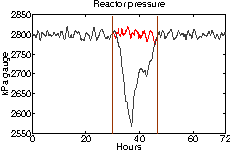
\includegraphics[height=3cm]{entropy_a}
            \caption{Manipulierte Werte des Reaktors}
            \label{fig:spoof}
        \end{subfigure}
        \begin{subfigure}[t]{0.4\textwidth}
            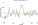
\includegraphics[height=3cm]{entropy_b}
            \caption{Entropie des gesamten Kraftwerks}
            \label{fig:entropy_success}
        \end{subfigure}
        \caption{Detektion eines Integrity-Angriffs~\cite{KLG15}}
        \label{fig:entropie}
    \end{figure}

    \citeauthor{CAS+09}~\cite{CAS+09} schlägt vor dem Betreiber von Kontrollsystemen genügend Informationen zukommen zu lassen um angemessen auf Anomalien zu reagieren.
    Abgesehen von menschlicher Interaktion sollten allerdings, gerade in Echtzeitsystemen, vor allem automatische Prozesse eine Wiederherstellung ermöglichen.

    In \cite{KXW+18} wird ein automatisches Verfahren zur Wiederherstellung vorgestellt.
    Hierbei werden Checkpoints der physischen- und Cyber-Systeme verwendet, um ein die Funktionsweise eines \cps wiederzustellen.
    Dieses Verfahren findet beispielsweise Anwendung bei manipulierten Sensoren.
    Dieses bieten einen Vorteil gegenüber Redundanz und Diversität, da auch wenn alle Sensoren kompromittiert sind, immer noch ein Betrieb sichergestellt werden kann.
    Die erfolgreichen Ergebnisse des Verfahrens wurden experimentell durch Simulationen und Test in einem Fahrzeug nachgewiesen.

    \section{Verbesserung der aktuellen Sicherheitssituation von \glsentryshort{cps}}
    \label{sec:improve-security-situation}

    \newpage
    % ~\nocite{*}

    \printbibliography
    \newpage
\end{document}
